\documentclass[../../main.tex]{subfiles}
\begin{document}

\begin{flushright}
  \footnotesize\textit{【自動文字起こし・要確認】}
\end{flushright}

[解] 題意の正八面体の一辺を $2$ とし，$P_1$ を始点とするベクトル $\overrightarrow{P_1 P_m}$ の終点を $\nabla$ とする．
任意の $m \ (m=2,\cdots,6)$ に対し
\[ \overrightarrow{P_1 P_m} \cdot \vec{v} \le 0 \]
を満たす $\nabla$ の存在範囲は，右図で $\overrightarrow{P_1 P_m}$ を法線ベクトルとする $(m=2,3,4,5)$ 4平面で囲まれた部分（$\alpha$ とおく）である．ところでこの4平面は，右下図のように空間を対称に $4$ 等分割するので，
（立方体の各面を底面，$P_1$ を頂点とする $6$ つの四角錐は合同）
対称性から $\nabla$ が $\alpha$ にある場合のみを考えれば良い．
又，題意から
\[ \overrightarrow{P_1 P_m} \cdot \vec{v} \neq 0 \]
である．以上から
\[ \overrightarrow{P_1 P_m} \cdot \vec{v} < 0 \]
となり，題意は示された．

\begin{figure}[htb]
  \centering
  % どちらも頂点を座標軸上の ±単位点とした正八面体．右は外接立方体の各面の中心を結ぶ．
  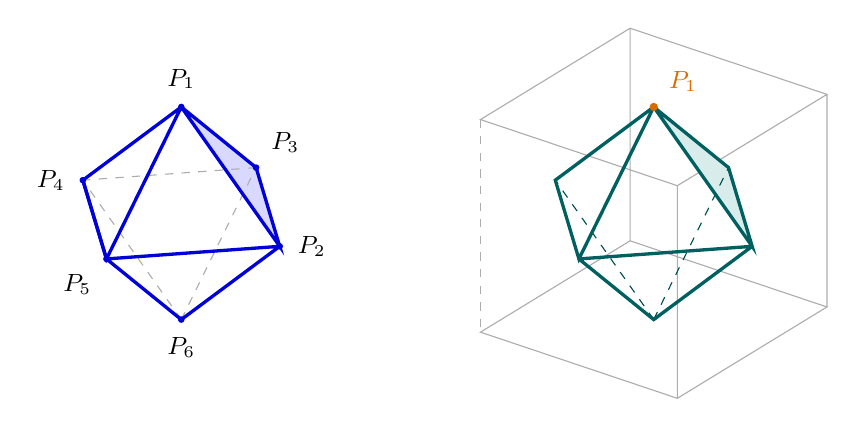
\begin{tikzpicture}[x={(1.25cm,-0.42cm)}, y={(0.95cm,0.58cm)},
    z={(0cm,1.35cm)}, >=stealth, every node/.style={font=\small}]
    \begin{scope}
      \coordinate (P1) at (0,0,1);
      \coordinate (P2) at (1,0,0);
      \coordinate (P3) at (0,1,0);
      \coordinate (P4) at (-1,0,0);
      \coordinate (P5) at (0,-1,0);
      \coordinate (P6) at (0,0,-1);
      \fill[blue!15] (P1) -- (P2) -- (P3) -- cycle;
      \draw[dashed, gray!65] (P6) -- (P3) (P6) -- (P4) (P3) -- (P4);
      \draw[line width=1.2pt, blue!85!black]
      (P1) -- (P2) -- (P3) -- (P1) -- (P4) -- (P5) -- (P1);
      \draw[line width=1.2pt, blue!85!black]
      (P2) -- (P5) -- (P4) (P2) -- (P6) -- (P5);
      \foreach \name in {P1,P2,P3,P4,P5,P6}
      \fill[blue!85!black] (\name) circle (1.2pt);
      \node[above=3pt] at (P1) {$P_1$};
      \node[right=3pt] at (P2) {$P_2$};
      \node[above right=2pt] at (P3) {$P_3$};
      \node[left=3pt] at (P4) {$P_4$};
      \node[below left=2pt] at (P5) {$P_5$};
      \node[below=3pt] at (P6) {$P_6$};
    \end{scope}
    \begin{scope}[shift={(6cm,0cm)}]
      \coordinate (A) at (1,1,1);
      \coordinate (B) at (-1,1,1);
      \coordinate (C) at (-1,-1,1);
      \coordinate (D) at (1,-1,1);
      \coordinate (E) at (1,1,-1);
      \coordinate (F) at (-1,1,-1);
      \coordinate (G) at (-1,-1,-1);
      \coordinate (H) at (1,-1,-1);
      \draw[gray!65, thin] (A) -- (B) -- (C) -- (D) -- cycle
      (A) -- (E) (B) -- (F) (D) -- (H)
      (E) -- (F) -- (G) -- (H) -- cycle;
      \draw[dashed, gray!65] (C) -- (G);
      \coordinate (Q1) at (0,0,1);
      \coordinate (Q2) at (1,0,0);
      \coordinate (Q3) at (0,1,0);
      \coordinate (Q4) at (-1,0,0);
      \coordinate (Q5) at (0,-1,0);
      \coordinate (Q6) at (0,0,-1);
      \fill[teal!15] (Q1) -- (Q2) -- (Q3) -- cycle;
      \draw[dashed, teal!60!black] (Q6) -- (Q3) (Q6) -- (Q4);
      \draw[teal!75!black, line width=1.2pt]
      (Q1) -- (Q2) -- (Q3) -- (Q1) -- (Q4) -- (Q5) -- (Q1)
      (Q2) -- (Q5) -- (Q4) (Q2) -- (Q6) -- (Q5);
      \fill[orange!85!black] (Q1) circle (1.5pt);
      \node[above right=2pt, orange!85!black] at (Q1) {$P_1$};
    \end{scope}
  \end{tikzpicture}
  \caption{正八面体の頂点と辺（左），各面の中心が正八面体の頂点となる外接立方体（右）}
\end{figure}

[解2] 正八面体の中心を $O$ とし，$\overrightarrow{OX} = \vec{v}$ となる点 $X$ をとる．$P_1, \cdots, P_6$ の中で点 $X$ から最も近い点を $P_k$ とする．$|P_k X| \le |P_m X|$ より
\[ |\overrightarrow{OX} - \overrightarrow{OP_k}| \le |\overrightarrow{OX} - \overrightarrow{OP_m}| \]
各辺 $0$ 以上だから $2$ 乗して
\begin{eqnarray*}
  2 (\overrightarrow{OP_m} - \overrightarrow{OP_k}) \cdot \overrightarrow{OX} &\le& |\overrightarrow{OP_m}|^2 - |\overrightarrow{OP_k}|^2 = 0 \\
  \therefore \overrightarrow{P_k P_m} \cdot \vec{v} &\le& 0
\end{eqnarray*}
$\overrightarrow{P_k P_m} \cdot \vec{v} \neq 0$ から
\[ \overrightarrow{P_k P_m} \cdot \vec{v} < 0 \]

\end{document}
